	\section{Цель работы}
		Изучить методы и средства автоматизированного реферирования и аннотирования текстов на естественном языке, а также получить навыки работы с подобными системами.
	\section{Основные понятия}
	
	Реферат (нем. Referat, от лат. refere — докладывать, сообщать) — доклад по определённой теме, в котором собрана информация из одного или нескольких источников. 
	Рефераты могут являться изложением содержания научной работы, статьи и т. п. 
	Реферат никак не соотносится с вторичным текстом, переписанным из первоисточника, поскольку это самостоятельная исследовательская работа, раскрывающая суть изучаемой темы. 
	Как правило, реферат отражает различные точки зрения на исследуемый вопрос, выражая в то же время и мнение самого автора.
	
	Аннотация (от лат. annotatio — замечание) или резюме (от фр. résumé — <<сокращённый>>) — краткое содержание книги или другого издания, а также краткая характеристика издания: рукописи, монографии, статьи или книги. 
	Аннотация показывает отличительные особенности и достоинства издаваемого, место и время издания в номинативной форме. 
	Аннотация содержит основную тему статьи или книги, кроме этого она может перечислять (называть) основные положения описываемого источника. 
	Аннотация может не упоминать субъект действия (предполагая, что он известен из контекста), и содержать пассивные конструкции — глагольные и причастные.
	
	\subsection{TextAnalyst}
	TextAnalyst разработан в качестве инструмента для анализа содержания текстов, смыслового поиска информации, формирования электронных архивов, и предоставляет пользователю следующие основные возможности: 
	
	\begin{itemize}
		\item анализа содержания текста с автоматическим формированием семантической сети с гиперссылками - получения смыслового портрета текста в терминах основных понятий и их смысловых связей; 
		\item анализа содержания текста с автоматическим формированием тематического древа с гиперссылками - выявления семантической структуры текста в виде иерархии тем и подтем; 
		\item смыслового поиска с учетом скрытых смысловых связей слов запроса со словами текста; 
		\item автоматического реферирования текста - формирования его смыслового портрета в терминах наиболее информативных фраз; 
		\item кластеризации информации - анализа распределения материала текстов по тематическим классам;
		\item автоматической индексации текста с преобразованием в гипертекст; 
		\item ранжирования всех видов информации о семантике текста по «степени значимости» с возможностью варьирования детальности ее исследования; 
		\item автоматического/автоматизированного формирования полнотекстовой базы знаний с гипертекстовой структурой и возможностями ассоциативного доступа к информации; 
	\end{itemize}
	
	Одна из возможностей TextAnalyst – построение сети понятий. 
	
	Сеть понятий - это множество терминов из текстов - слов и словосочетаний, связанных между собой по смыслу. 
	В сеть включены не все термины текста, а лишь наиболее значимые, несущие основную смысловую нагрузку. 
	Каждый элемент сети - понятие характеризуется числовой оценкой – так называемым смысловым весом. 
	Связи между парами понятий, в свою очередь, также характеризуются весами. 
	Эти оценки позволят сравнить относительный вклад различных понятий и их связей в семантику текста, выявить более или менее подробно проработанную в тексте тематику, задать способ сортировки информации, и, наконец, позволят взглянуть на весь текстовый материал по пластам - смысловым срезам различной глубины - то <<снимая сливки>> с содержания, то глубоко погружаясь в детали. 
	
	Другая возможность TextAnalyst – построение тематической структуры текста. 
	
	Тематическая структура описывает содержание анализируемых текстов в виде иерархии связанных тем и подтем. 
	Все темы и подтемы выражены в терминах исходных текстов и соответствуют узлам сети понятий. 
	Однако связи между понятиями односторонни и направлены от главного понятия к подчиненным. 
	Тематическая структура, таким образом, имеет вид древа, в корне которого стоят главные темы, в ветвях – их подтемы, и каждая ветвь дерева заканчивается. 
	
	
	\section{Порядок выполенения работы}
			
			
			\subsection{Работа с художественным текстом}
				В качестве художественного рассмотрим \href{./listings/chipollino-source.txt}{первые 10 глав сказки <<Приключения Чиполлино>>} итальянского писателя Джанни Родари.
				Ограничение в 10 глав принято из-за ограничений бесплатной версии программы.
				Общая длина текста - 2272 предложения.
			
			\begin{figure*}[h]
				\centering
				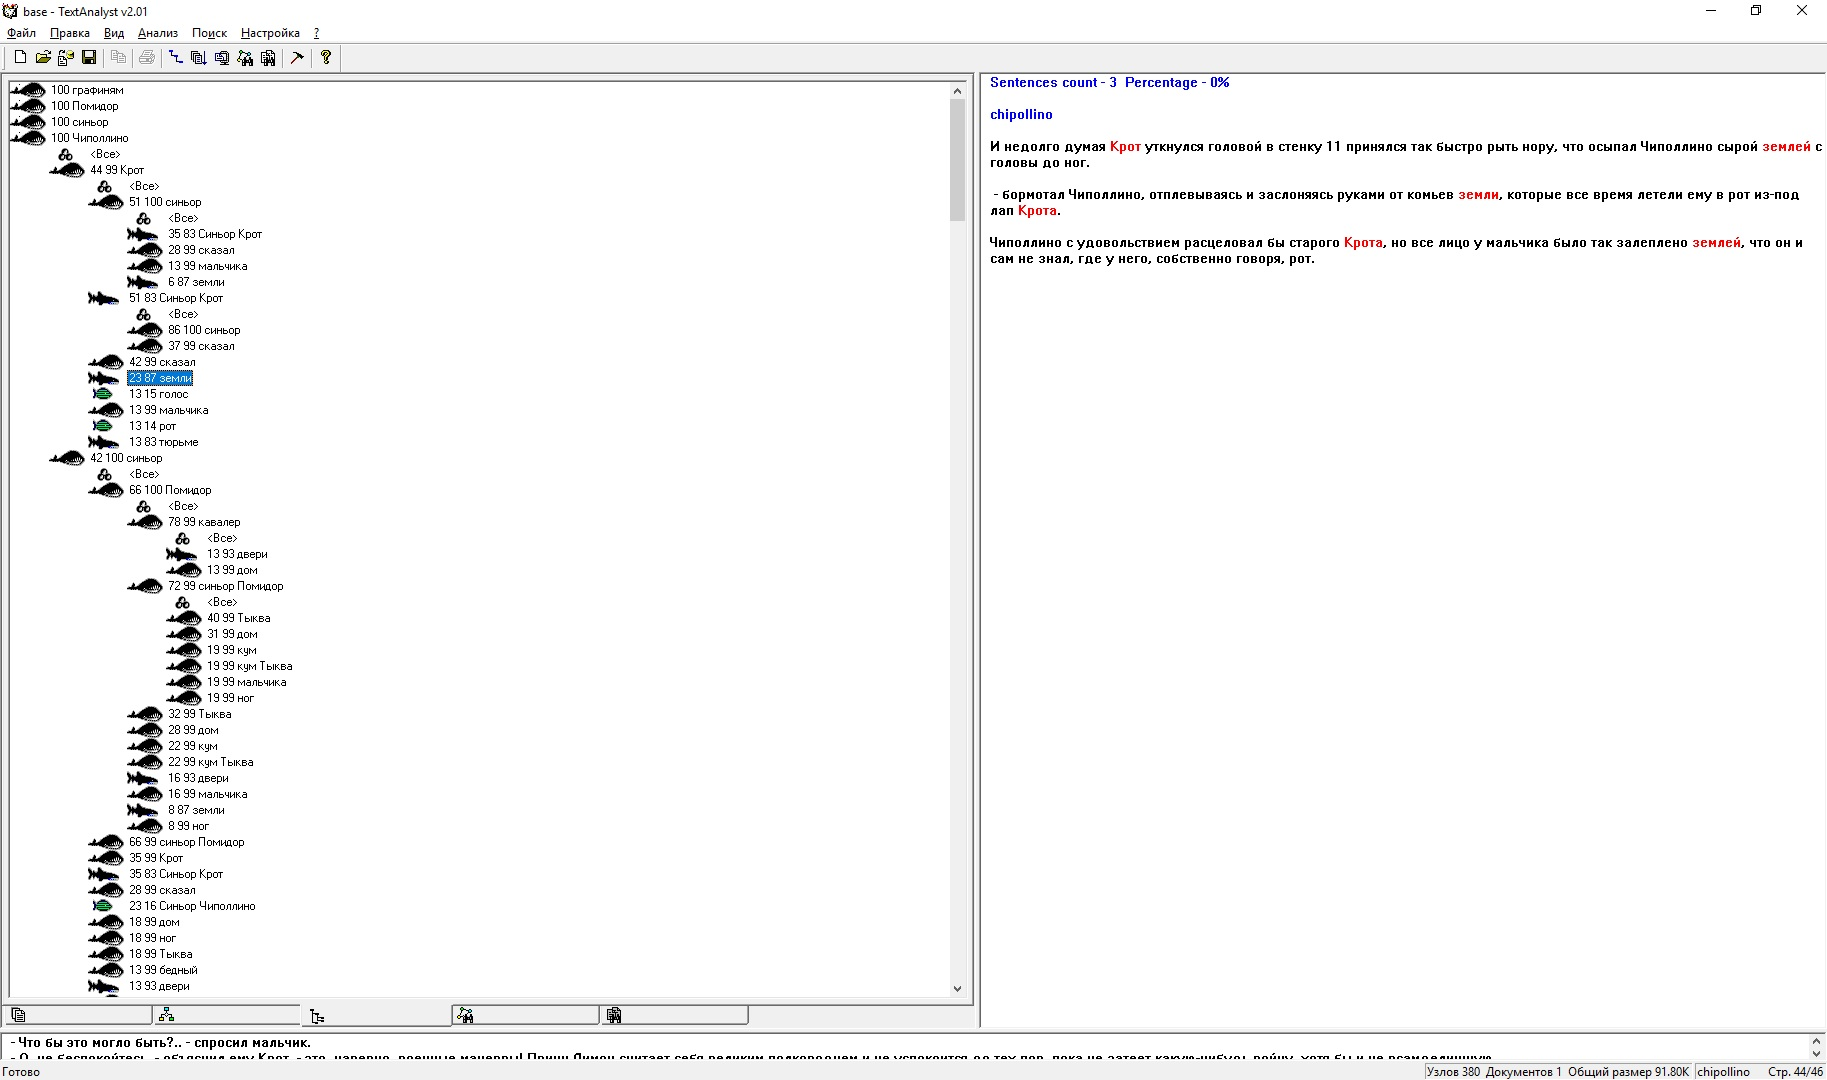
\includegraphics[width=0.7\linewidth]{images/semantic-net}
				\caption{Фрагмент семантической сети произведения <<Приключения Чиполлино>>}
				\label{fig:semantic-net}
			\end{figure*}
			\begin{figure*}[h]
				\centering
				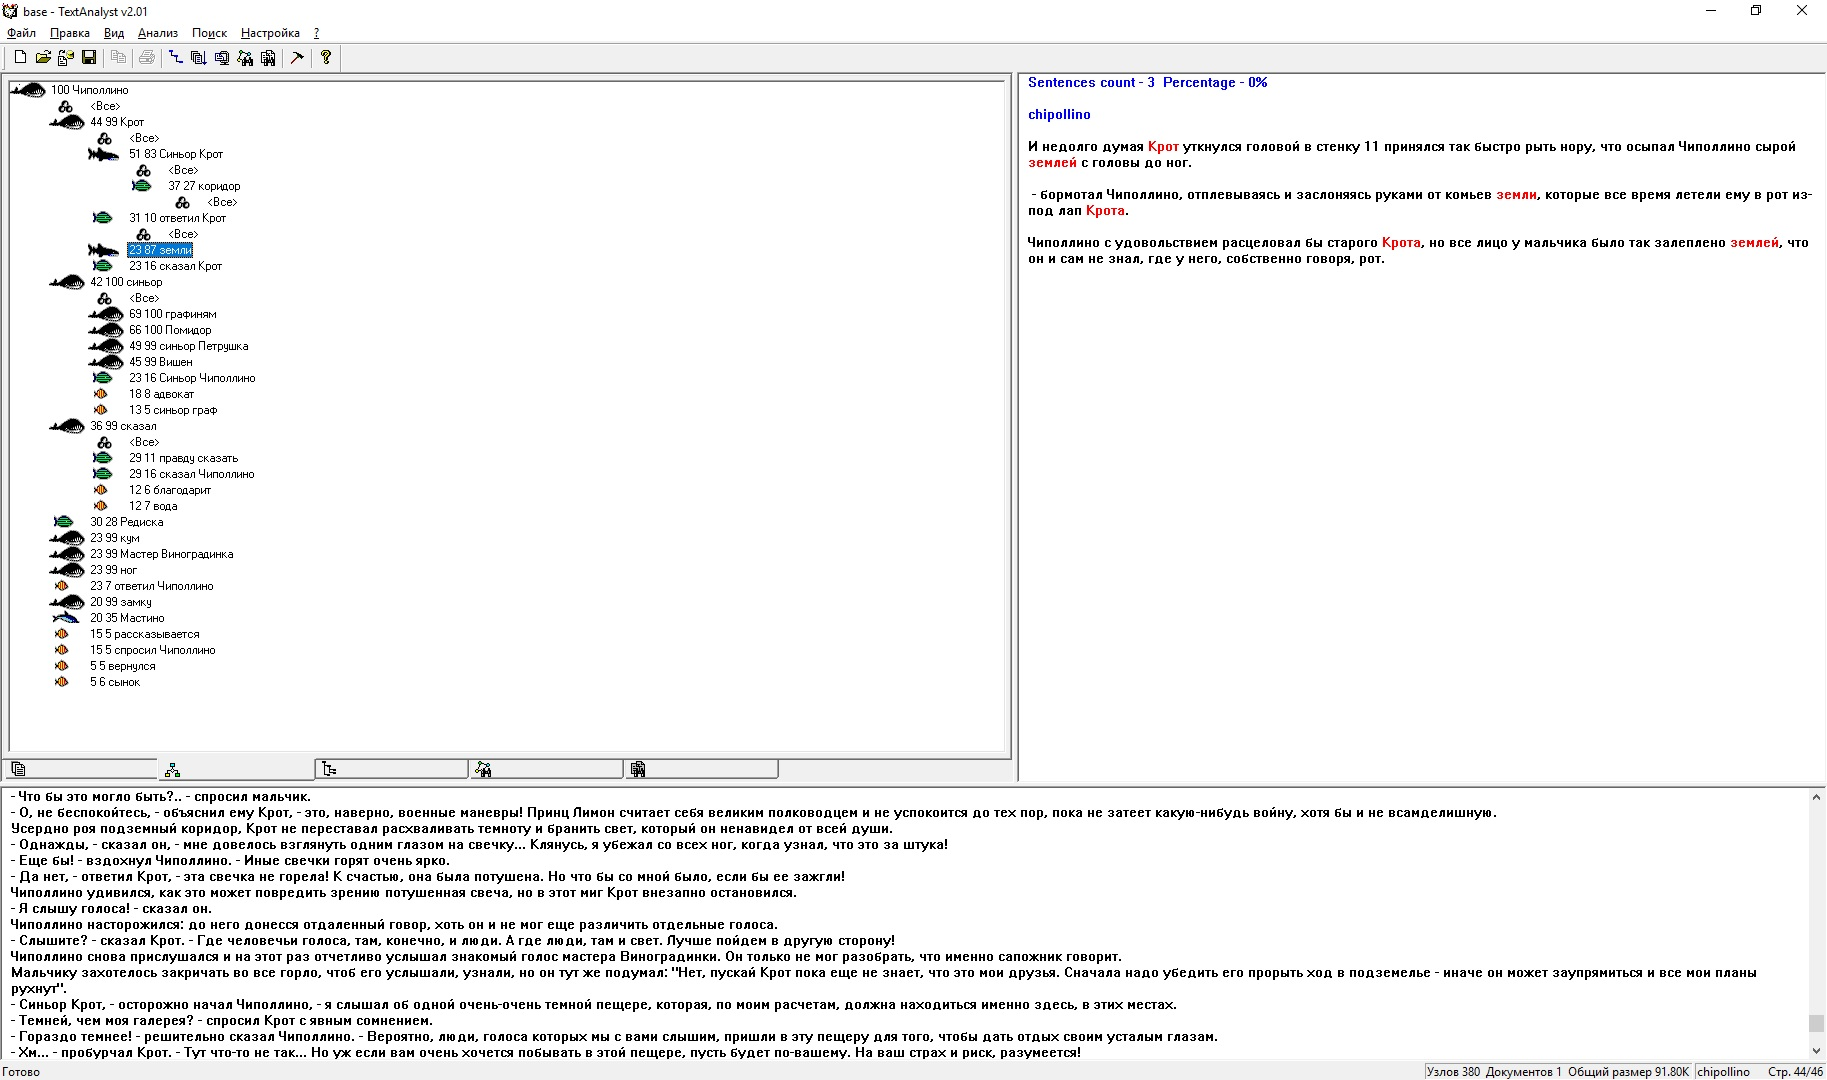
\includegraphics[width=0.7\linewidth]{images/chipollino-theme-tree}
				\caption{Фрагмент тематического дерева произведения <<Приключения Чиполлино>>}
				\label{fig:chipollino-theme-tree}
			\end{figure*}
	
		\FloatBarrier
			
		\begin{table} [htbp]
			\centering
			\caption{Результаты автоматического реферирования}
			\label{table:trio}%
			\resizebox{\textwidth}{!}{%
				\begin{tabular}{|c|c|c|l|}
					\hline 
					Минимальный вес слова & Количество предложений & Размер текста,\% & Реферат \\
					\hline
					90 & 134 & 15 & \href{./listings/chipollino-result.txt}{Автореферат}\\
					\hline
					70 & 234 & 24 & \href{./listings/chipollino-result70.txt}{Автореферат}\\
					\hline
					30 & 379 & 37 & \href{./listings/chipollino-result30.txt}{Автореферат}\\
					\hline
			\end{tabular}}
		\end{table}
	
		Автореферат сносно передаёт значение каждой главы.
		Замечен интересный результат: в реферате присутствует большинство названий глав. 
		Например, название первой главы: <<\textit{в которой Чиполлоне отдавил ногу принцу Лимону}>>.
		Таким образом, краткое описание, данное автором, верно оценивается программой, как наиболее информативное.
		
		\href{./listings/chipollino.html}{Cемантическая сеть}
		
		\subsection{Автоматическое реферирование технического текста}
		В качестве примера рассмотрим работу с \href{./listings/lab-3.txt}{текстом задания к лабораторной работе}.
		Размер документа - 149 предложений.
		
				
		\begin{figure*}[h]
			\centering
			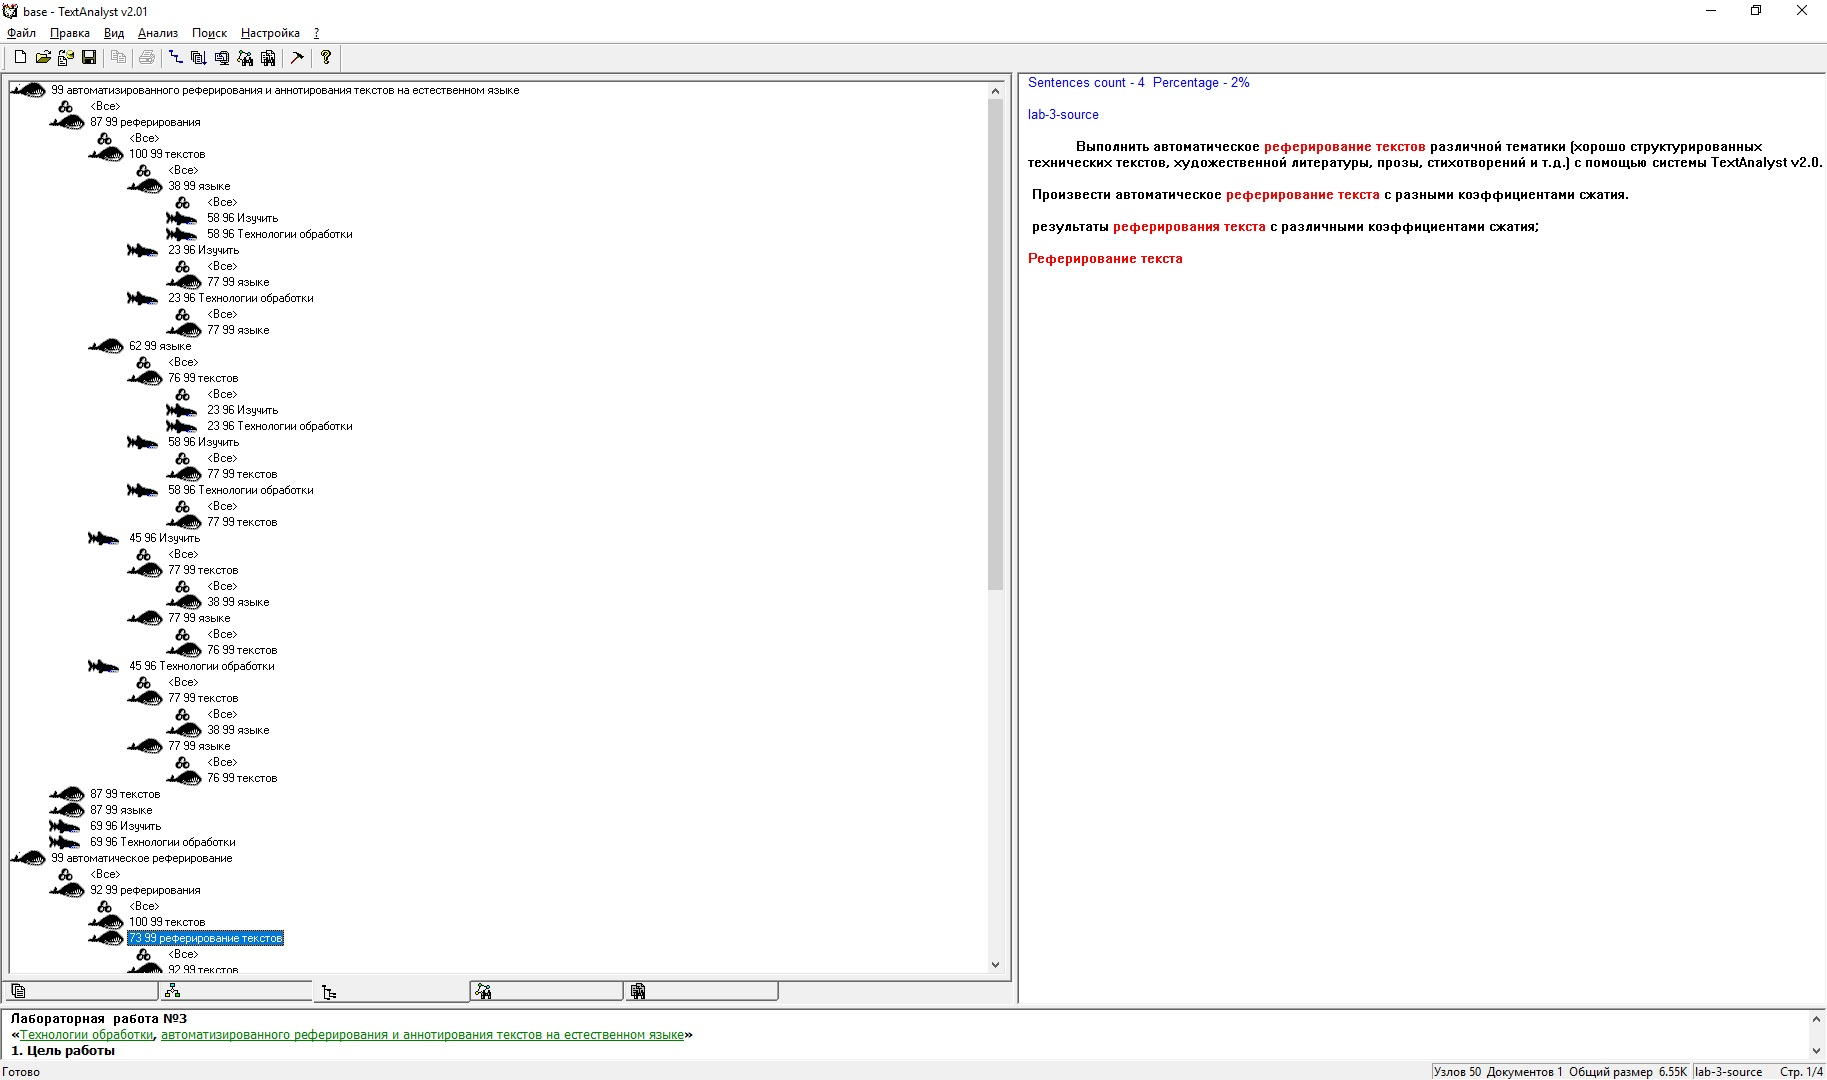
\includegraphics[width=0.7\linewidth]{images/lab-3-semantic-net}
			\caption{Фрагмент семантической сети}
			\label{fig:lab-3-semantic-net}
		\end{figure*}
	
	
		
		\begin{figure*}[h]
			\centering
			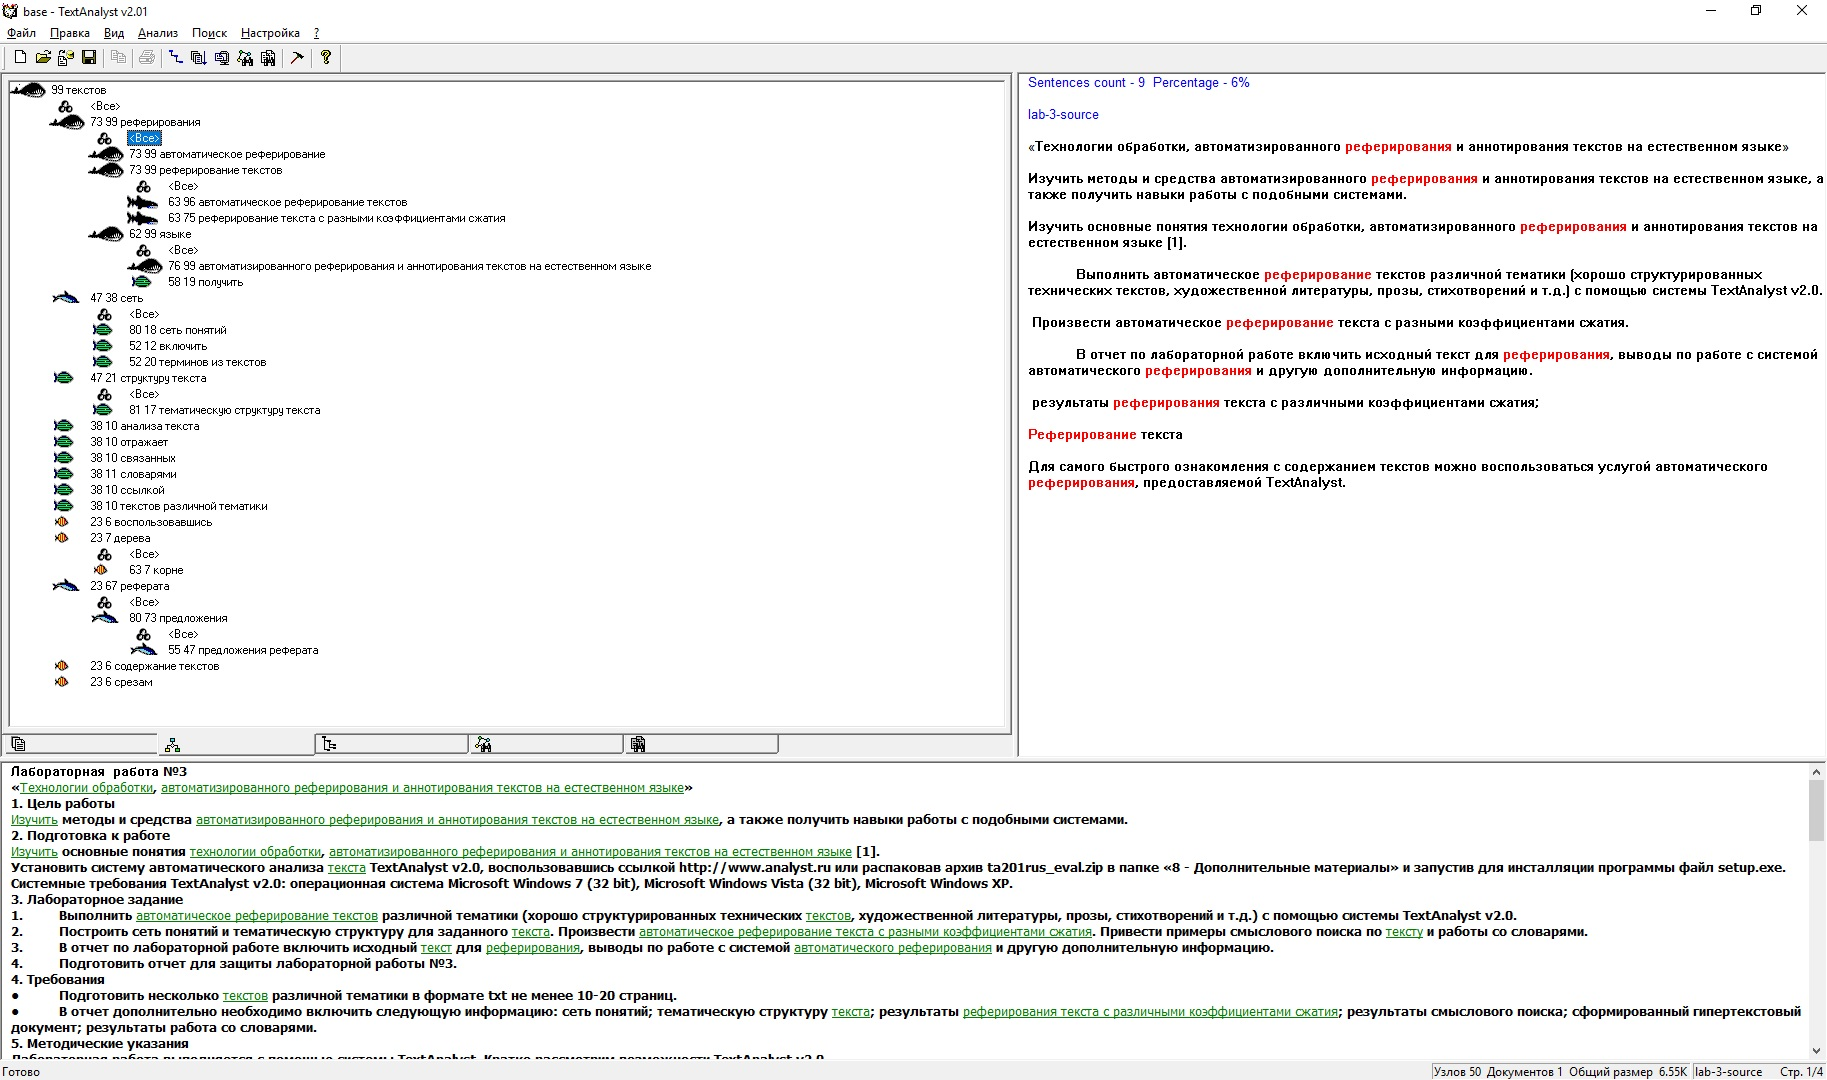
\includegraphics[width=0.7\linewidth]{images/lab-3-theme-tree}
			\caption{Фрагмент тематического дерева}
			\label{fig:lab-3-theme-tree}
		\end{figure*}

		\begin{table} [htbp]
			\centering
			\caption{Результаты автоматического реферирования текста задания}
			\label{table:lab}%
			\resizebox{\textwidth}{!}{%
				\begin{tabular}{|c|c|c|l|}
					\hline 
					Минимальный вес слова & Количество предложений & Размер текста,\% & Реферат \\
					\hline
					90 & 6 & 11 & \href{./listings/lab-3-result.txt}{Автореферат}\\
					\hline
					70 & 11 & 20 & \href{./listings/lab-3-result70.txt}{Автореферат}\\
					\hline
					30 & 12 & 23 & \href{./listings/lab-3-result30.txt}{Автореферат}\\
					\hline
			\end{tabular}}
		\end{table}
	
	\href{./listings/lab-3.html}{Cемантическая сеть}
	
	Получившиеся рефераты мало отличаются.
	При этом все они достаточно точно передают общую суть работы - произвести автоматическое реферирование.
	Однако реферат плохо раскрывает детали.
	Включенными оказались предложения, в которых много основных понятий.
	
	\section{t-CONSPECTUS}
	\href{http://tconspectus.pythonanywhere.com/summarization}{t-CONSPECTUS} - это саммарайзер экстрактного типа, т.е. он формирует реферат из предложений оригинальной статьи, которые в процессе анализа получили наибольший вес, и, следовательно, лучше всего передают смысл содержимого. На сайте можно использовать не только оригинальный метод реферирования, но и сравнить его с другими распространёнными алгоритмами, например, TextRank.
	
	Ресурс позволяет также произвести взвешивание слов в тексте.
	Алгоритм использует словарь русского языка и автоматически определяет разные словоформы.
	Доступно множество различных метрик.
	
	Вся информация об алгоритме и возможностях программы представлена на официальном сайте.
	
	Для сравнения произведено реферирование  \href{./listings/chipollino-conspectus.txt}{художественного текста} и \href{./listings/lab-3-conspectus.txt}{технического текста} с коэффициентом сжатия 15\%. 
	Художественный текст стал менее связен и понятен, также в него не вошли названия глав.
	Технический текст, напротив, включил необходимый минимум.
	
	\section{Вывод}
	Программа TextAnalyst позволяет анализировать тексты различной тематики, структуры, строить сеть понятий и производить автореферирование. 
	Программа обладает простым, но устаревшим пользовательским интерфейсом. 
	Существует ограничение для бесплатной версии: позволяет открывать файлы, размер которых не превышает 100кб, что существенно усложнило подбор текстов в формате .rtf для выполнения данной лабораторной работы. 
	
	Рассмотрено веб-саммарайзер t-CONSPECTUS - современный аналог TextAnalyst.
	